
%\documentclass[12pt]{amsart}
%\usepackage{geometry} % see geometry.pdf on how to lay out the page. There's lots.
%\usepackage{datetime}
%\usepackage{setspace}
%\doublespacing
%\geometry{a4paper} % or letter or a5paper or ... etc
%% \geometry{landscape} % rotated page geometry
%
%% See the ``Article customise'' template for come common customisations
%
%\title{Wind chapter}
%\author{Percy Link}
%\date{\currenttime \ \today} % delete this line to display the current date
%
%%%% BEGIN DOCUMENT
%\begin{document}
%
%\maketitle

\section{Results}

We first characterize the differences in Solano turbine-level wind resulting from the soil moisture tests (Section \ref{subsec:CharWindChanges}).  We then investigate the physical mechanism linking changes in soil moisture to changes in Solano wind timing and magnitude (Section \ref{subsec:PhysMech}).

\subsection{Characterization of Solano wind sensitivity to soil moisture}
\label{subsec:CharWindChanges}

\subsubsection{California low-level wind system}
\label{subsubsec:control_winds}

%Before presenting the Solano winds, we quantify the synoptic and land-surface-heating forcing in each case, and we characterize the control case winds.  The synoptic forcing, measured by wind speed at 500 hPa, varies little between the model runs (Figure \ref{fig:windSol_forcings}), and synoptic winds are weak on June 27 to July 5 and strong on July 6 to 11.  In all three regions, land surface sensible heat flux is approximately 200 W/m$^2$ greater at midday with wet soil moisture (0.25) than dry soil moisture (0.1).

The low-level winds in California follow a strong diurnal cycle, driven by the diurnal cycle of the temperature difference and thus the pressure difference between land and ocean.  Regional low-level winds in the control case are consistent with previous studies of California surface winds (Figure \ref{fig:windSol_WindMapsRg} first column, Zhong \textit{et al.}, 2004; Mansbach, 2010); flow is strong through the Solano pass and splits into northward and southward branches in the Central Valley.  The southward branch is stronger than the northward branch at 06:00 and 14:00, and the northward branch strengthens at 18:00 and 00:00.  The pressure gradient from the San Francisco Bay to the Central Valley remains strong from 14:00 to 00:00 and weakens by 06:00.  \textbf{Note: I need to remake these plots to label the pressure change contours.}

\begin{figure}[here]
\includegraphics[angle=90,origin=c,width=1\textwidth]{ch3-wind/img/wind_map_regions2.eps}
\caption{Wind speed (color shading) and direction (vectors) and pressure (color contours) at 110 m ASL on the d02 domain, averaged by hour over the two-week runs.  (a)-(d) CA-0.25 control case.  (e)-(h) dryCR case, changes in wind and pressure.  (i)-(l) dryCV case, changes in wind and pressure.  (m)-(p) drySN case, changes in wind and pressure.  Top row: average for hour 06:00 for the whole run; second row: average for hour 14:00; third row: average for hour 18:00; bottom row: average for hour 00:00.}
\label{fig:windSol_WindMapsRg}
\end{figure}

\begin{figure}[here]
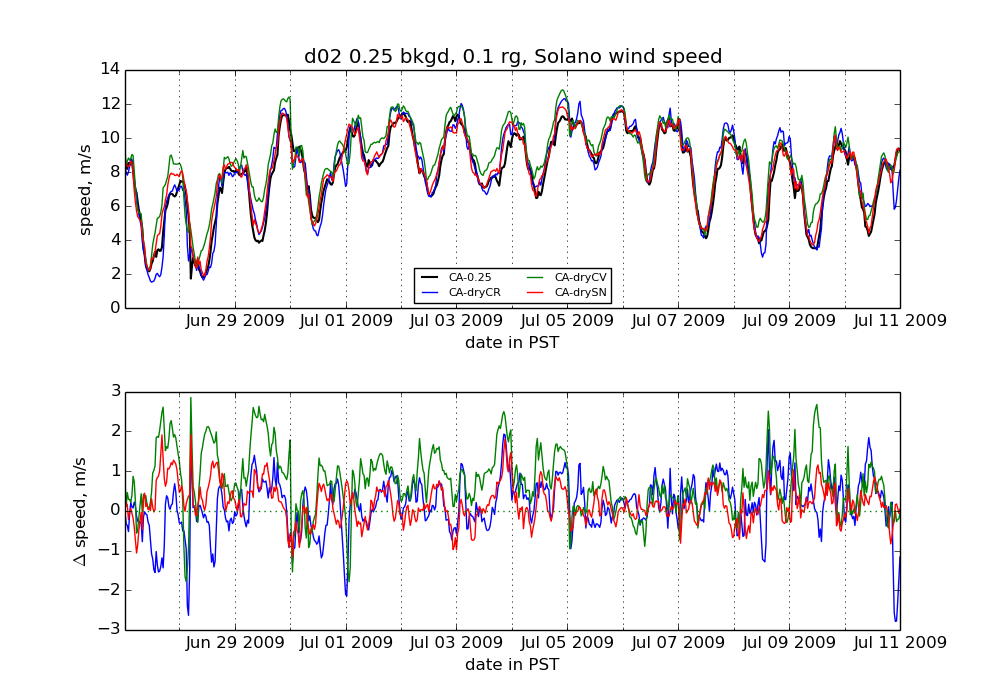
\includegraphics[width=1\textwidth]{ch3-wind/img/solano_wind_wetbkd_dryrg_d02_level0.png}
\caption{Time series of wind speed magnitude at 60 m AGL for the d02 grid point nearest the Solano wind farm, for the wet background and dry perturbation tests.  The model spin-up period is excluded.}
\label{fig:windSol_TseriesDryRg}
\end{figure}

\begin{figure}[here]
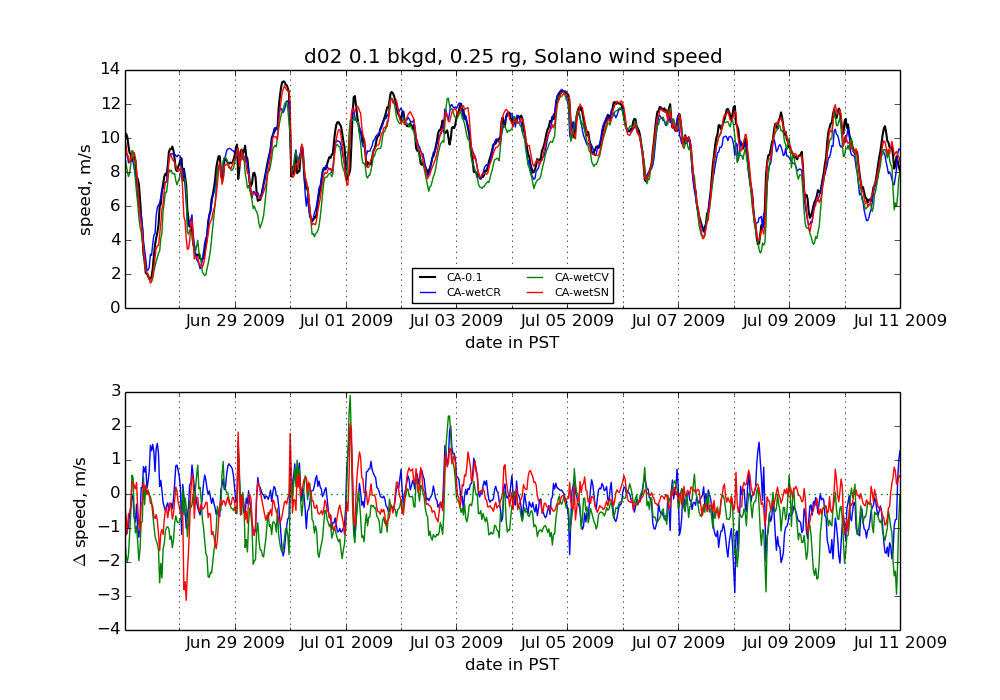
\includegraphics[width=1\textwidth]{ch3-wind/img/solano_wind_drybkd_wetrg_d02_level0.png}
\caption{Time series of wind speed magnitude at 60 m AGL for the d02 grid point nearest the Solano wind farm, for the dry background and wet perturbation tests.  The model spin-up period is excluded.}
\label{fig:windSol_TseriesWetRg}
\end{figure}

Similarly, wind at Solano has a strong diurnal cycle (Figures \ref{fig:windSol_TseriesDryRg}(a) and \ref{fig:windSol_TseriesWetRg}(a)); notably, the surface wind speed does not track the 500 hPa synoptic wind in this period (cf. Figure \ref{fig:windSol_forcings}) but rather is dominated by the diurnal signal.  Solano wind speeds are greatest at night (19:00 to 03:00) and weakest in the morning (08:00 to 13:00; Figure \ref{fig:windSol_DiffDiurnalDryRg}(a) and Figure \ref{fig:windSol_DiffDiurnalWetRg}(a))  There is a pronounced low-level ($\le$300 m) peak in Solano winds that is particularly pronounced at night (Figure \ref{fig:windSol_VertProfileDryRg}(a)).

\begin{figure}[here]
\begin{subfigure}{0.5\textwidth}
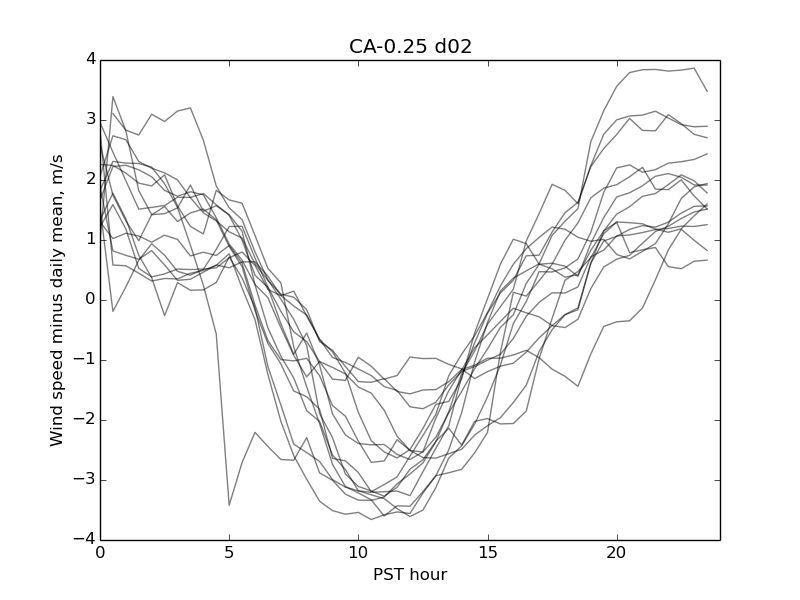
\includegraphics[width=1\textwidth]{ch3-wind/img/solano_controlwind_minusmean_CA0pt25_d02_level0.png}
\caption{}
\end{subfigure}
\begin{subfigure}{0.5\textwidth}
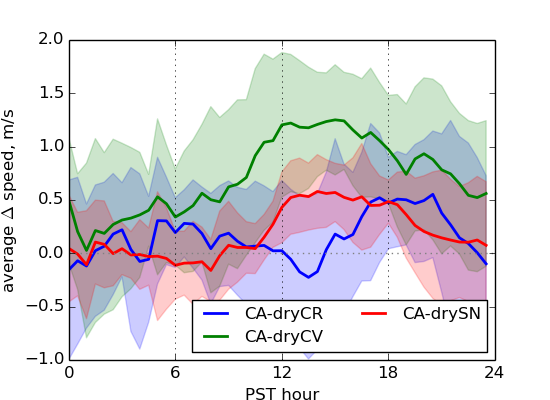
\includegraphics[width=1\textwidth]{ch3-wind/img/solano_diurnalwind_dry_regions_d02_level0.png}
\caption{}
\end{subfigure}
\caption{(a) Overlaid diurnal cycles of wind speed magnitude minus daily mean wind speed, at 60 m AGL for the d02 grid point nearest the Solano wind farm, for the CA-0.25 control case.  (b) Diurnally averaged differences in wind speed, at 60 m AGL for the d02 grid point nearest the Solano wind farm, for the wet background/dry perturbation cases.  Shading represents one standard deviation.}
\label{fig:windSol_DiffDiurnalDryRg}
\end{figure}

\begin{figure}[here]
\begin{subfigure}{0.5\textwidth}
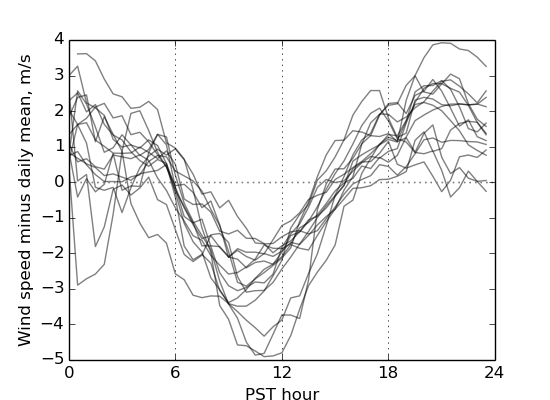
\includegraphics[width=1\textwidth]{ch3-wind/img/solano_controlwind_minusmean_CA0pt1_d02_level0.png}
\caption{}
\end{subfigure}
\begin{subfigure}{0.5\textwidth}
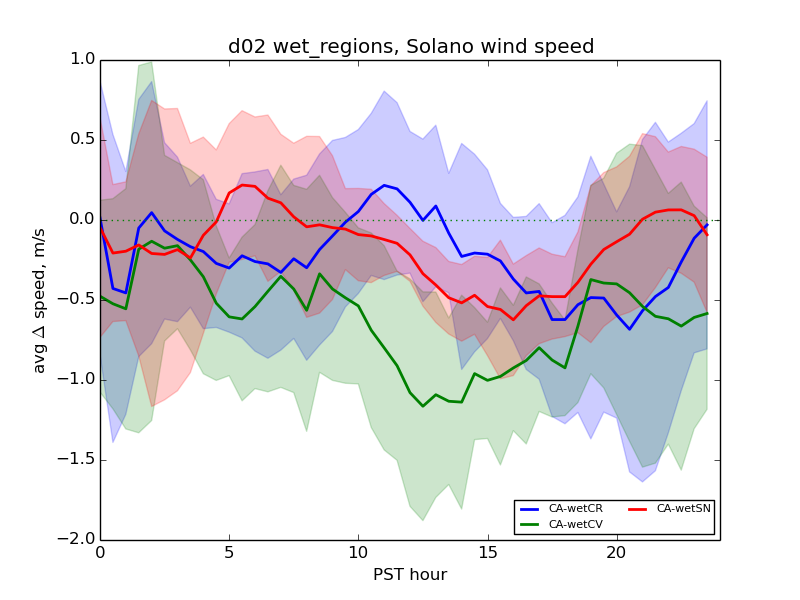
\includegraphics[width=1\textwidth]{ch3-wind/img/solano_diurnalwind_wet_regions_d02_level0.png}
\caption{}
\end{subfigure}
\caption{(a) Overlaid diurnal cycles of wind speed magnitude minus daily mean wind speed, at 60 m AGL for the d02 grid point nearest the Solano wind farm, for the CA-0.1 control case.  (b) Diurnally averaged differences in wind speed, at 60 m AGL for the d02 grid point nearest the Solano wind farm, for the dry background/wet perturbation cases.  Shading represents one standard deviation.}
\label{fig:windSol_DiffDiurnalWetRg}
\end{figure}

\begin{figure}[here]
\begin{subfigure}{0.49\textwidth}
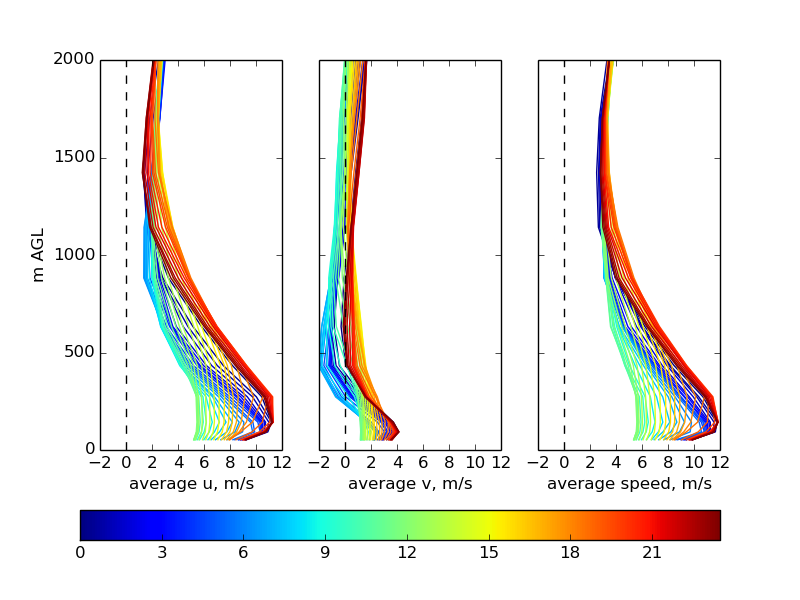
\includegraphics[width=\textwidth]{ch3-wind/img/windprof_hr_avg_CA0pt25.png}
\caption{}
\end{subfigure}
\begin{subfigure}{0.49\textwidth}
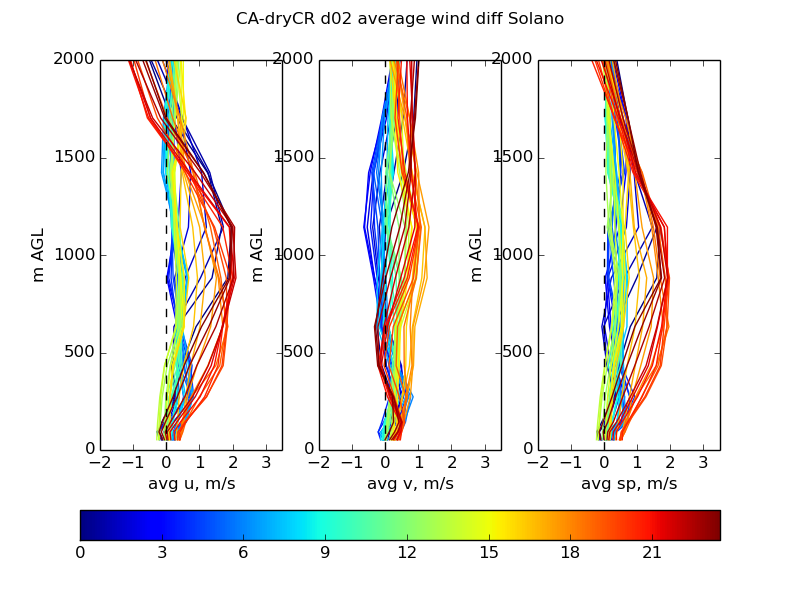
\includegraphics[width=\textwidth]{ch3-wind/img/windprof_diff_hr_avg_dryCR.png}
\caption{}
\end{subfigure}
\begin{subfigure}{0.49\textwidth}
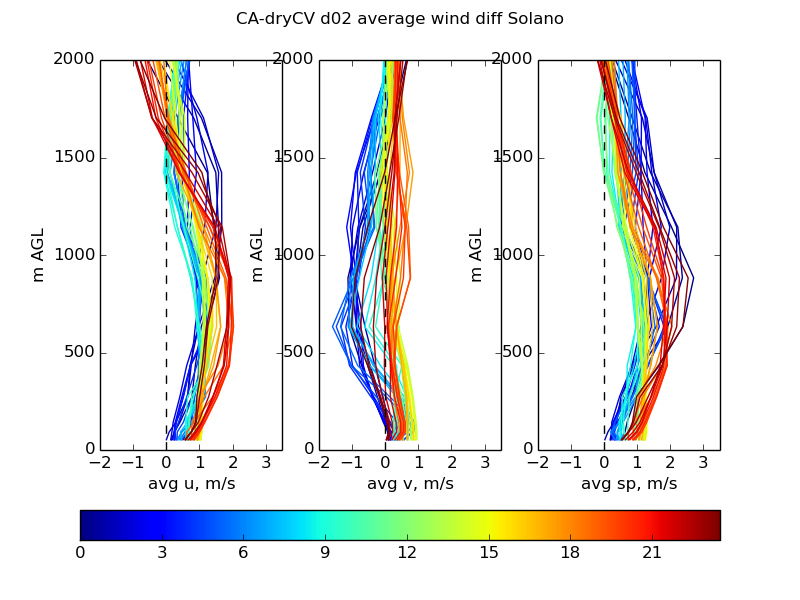
\includegraphics[width=\textwidth]{ch3-wind/img/windprof_diff_hr_avg_dryCV.png}
\caption{}
\end{subfigure}
\begin{subfigure}{0.49\textwidth}
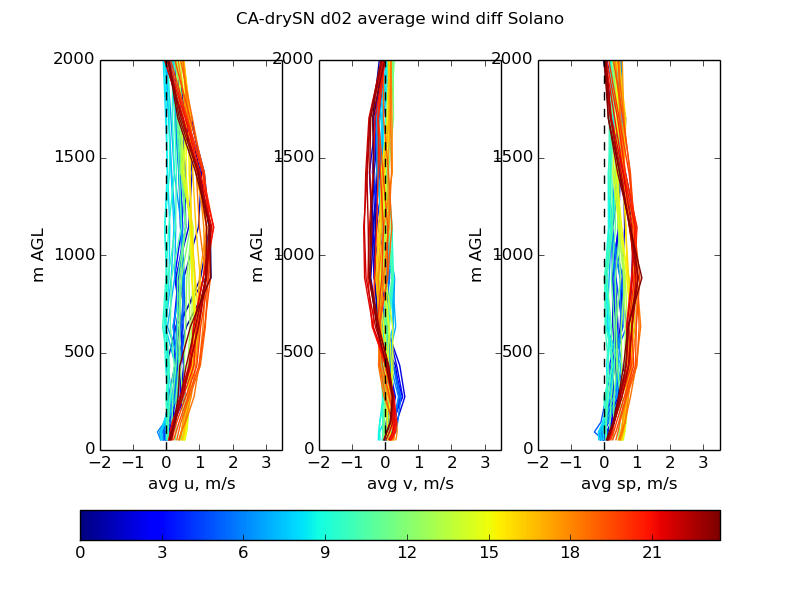
\includegraphics[width=\textwidth]{ch3-wind/img/windprof_diff_hr_avg_drySN.png}
\caption{}
\end{subfigure}
\caption{Vertical profiles of $u$, $v$, and $|u|$, averaged by time of day over the whole simulation (colorbar indicates hour of day in local time), for (a) CA-0.25 control run, and averaged differences from control run for the dry regional test cases: (b) dryCR, (c) dryCV, (d) drySN.}
\label{fig:windSol_VertProfileDryRg}
\end{figure}

\subsubsection{Regional sensitivity}

The Solano wind changes occur in the context of larger regional wind and pressure changes (Figure \ref{fig:windSol_WindMapsRg}).  In all dry regional tests, the pressure gradient and wind increase throughout the Central Valley, most strongly in the afternoon (second and third rows in Figure \ref{fig:windSol_WindMapsRg}).  In the dry Coast Range test (Figure \ref{fig:windSol_WindMapsRg} (e)-(h)), the pressure in the northern Central Valley decreases and wind in the northern Central Valley strengthens as cyclonic flow develops around the northern Coast Range.  In the dry Central Valley test (Figure \ref{fig:windSol_WindMapsRg} (i)-(l)), the pressure gradient from the San Francisco Bay to the Central Valley increases dramatically at 14:00, and these increases persist at 18:00 and to a lesser degree at 00:00. However, at 18:00, the zone of steepest pressure change has been pushed further eastward, and the strongest wind increases track this band of largest pressure gradient.  The pattern of wind increases at 00:00 is disorganized, and wind speeds decrease in the southern Central Valley at 06:00.  In the dry Sierra Nevada case (Figure \ref{fig:windSol_WindMapsRg} (m)-(p)), the pressure gradient strengthens moderately at 14:00 and 18:00, but pressure changes are minimal by 00:00 and 06:00.  Wind speeds increase through the Solano pass and the middle Central Valley in the afternoon (14:00 and 18:00), and by 18:00, the bands of largest wind increases have moved outward along Central Valley, again following zones of greatest pressure gradient increase.  Wind changes at night (00:00 and 06:00) are small and disorganized.

%The Solano wind in the regional test cases differs from the control case by as much as 2 m/s, and the largest changes occur when Central Valley soil moisture is perturbed (dryCV and wetCV).  

For all regional test cases, drier soils on a wet background increase Solano winds in the afternoon and evening relative to the all-wet control (Figure \ref{fig:windSol_DiffDiurnalDryRg}(b)); this increase is largest in the dryCV case.  The increases in both the dryCV and drySN cases are greatest between 11:00 and 18:00 (0.8-1.8 m/s for dryCV and 0.25-0.8 m/s for drySN), while the increase in the dryCR case happens later, between 17:00 and 22:00 (0.25-1 m/s).  Importantly, increases in the afternoon cause the daily wind speed ramp-up to shift earlier, because the increases occur at the same time as the control ramp-up (Figure \ref{fig:windSol_DiffDiurnalDryRg}(a)).  Because there are no corresponding decreases at the hour of ramp-down, this means that the duration of the high-wind period also increases.  Also, drier soils (especially in the Central Valley) increase the minimum wind (08:00 to 13:00) on many individual days (Figure \ref{fig:windSol_TseriesDryRg}), but the average increases in the minimum wind are not more than one standard deviation greater than zero in the two-week average diurnal cycle (Figure \ref{fig:windSol_DiffDiurnalDryRg}(b)).

Wetter soils on a dry background cause winds to decrease relative to the all-dry control case, and the magnitudes of the decreases are similar to the magnitudes of the increases in the dry regional tests (Figure \ref{fig:windSol_DiffDiurnalWetRg}(b)).  Again, the decrease is largest in when Central Valley soil moisture is perturbed.  Both the wetCV and wetSN cases have wind decreases during 10:00-18:00 that are more than one standard deviation from zero (0.5-1.8 m/s for wetCV and 0.25-0.8 m/s for wetSN); for the wetCR case, there are no times of day with wind changes more than one standard deviation from zero, although there are weak decreases in the late afternoon and evening.

In summary, the Central Valley soil moisture influences the Solano turbine-level winds more strongly than does the Coast Range or Sierra Nevada soil moisture.  Drier soils in all regions, but especially in the Central Valley, increase Solano wind speeds during ramp-up and peak hours (afternoon and evening); drier soils in the Central Valley, especially, shift the daily wind ramp-up earlier.  Conversely, wetter Central Valley soils cause Solano winds to decrease during ramp-up and peak times.

\subsubsection{Scaling of wind changes with Central Valley soil moisture}

\begin{figure}[here]
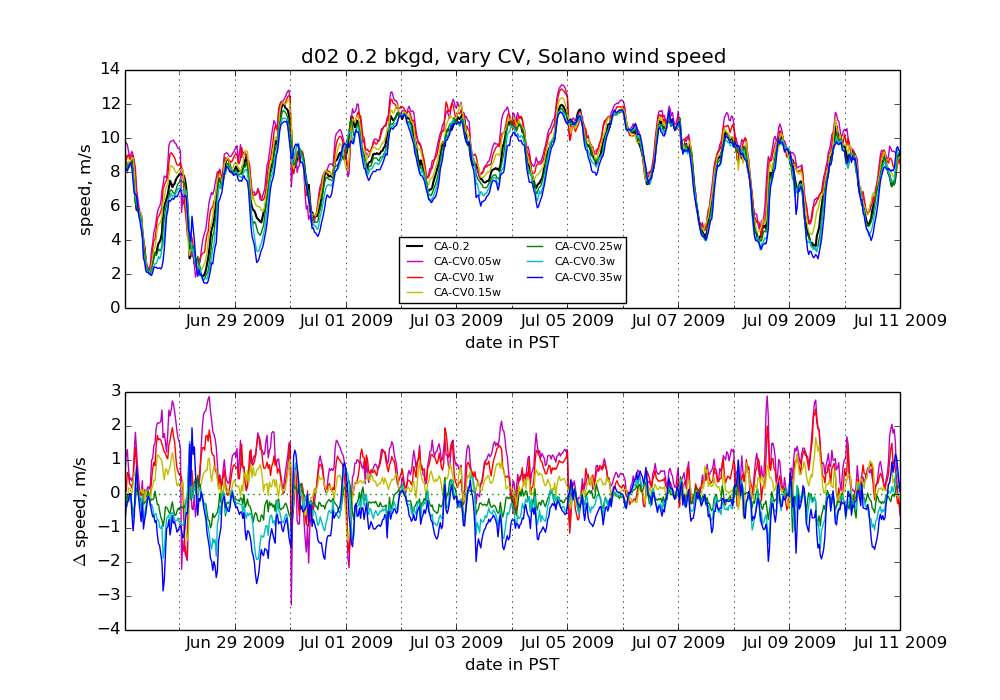
\includegraphics[width=1\textwidth]{ch3-wind/img/solano_wind_CV0pt2_d02_level0.png}
\caption{Time series of wind speed magnitude at 60 m AGL for the d02 grid point nearest the Solano wind farm, for a range of Central Valley soil moisture values, with soil moisture = 0.2 in the Coast Range and Sierra Nevada.  (a) Wind speed time series, (b) time series of differences between test cases and control (CA-0.2).  The model spin-up period is excluded.}
\label{fig:windSol_TseriesWindCV}
\end{figure}

\begin{figure}[here]
\begin{subfigure}{0.6\textwidth}
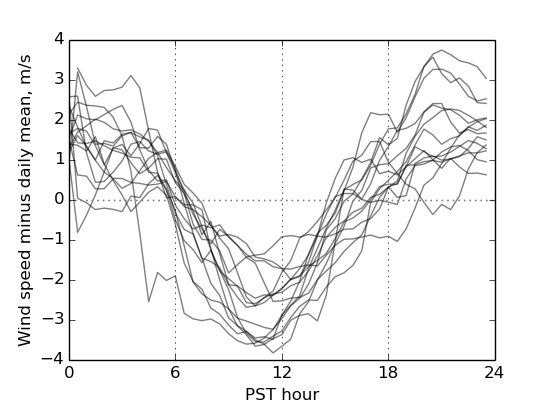
\includegraphics[width=1\textwidth]{ch3-wind/img/solano_controlwind_minusmean_CA0pt2_d02_level0.png}
\caption{}
\end{subfigure}
\begin{subfigure}{0.6\textwidth}
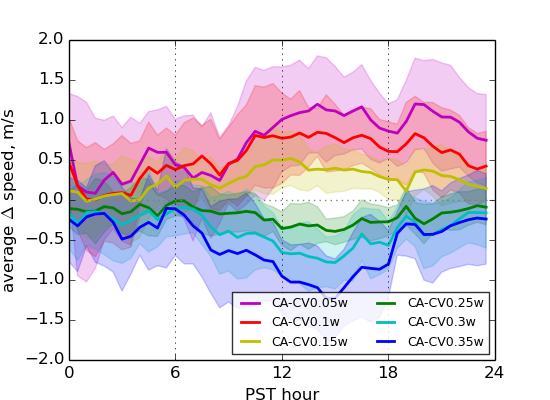
\includegraphics[width=1\textwidth]{ch3-wind/img/solano_diurnalwind_CV_0pt2_d02_level0.png}
\caption{}
\end{subfigure}
\caption{(a) Overlaid diurnal cycles of wind speed magnitude minus daily mean wind speed, at 60 m AGL for the d02 grid point nearest the Solano wind farm, for the CA-0.2 control case.  (b) Diurnally averaged differences in wind speed, at 60 m AGL for the d02 grid point nearest the Solano wind farm, for a range of Central Valley soil moisture values.  Shading represents one standard deviation.}
\label{fig:windSol_DiffDiurnalCV0pt2}
\end{figure}

\begin{figure}[here]
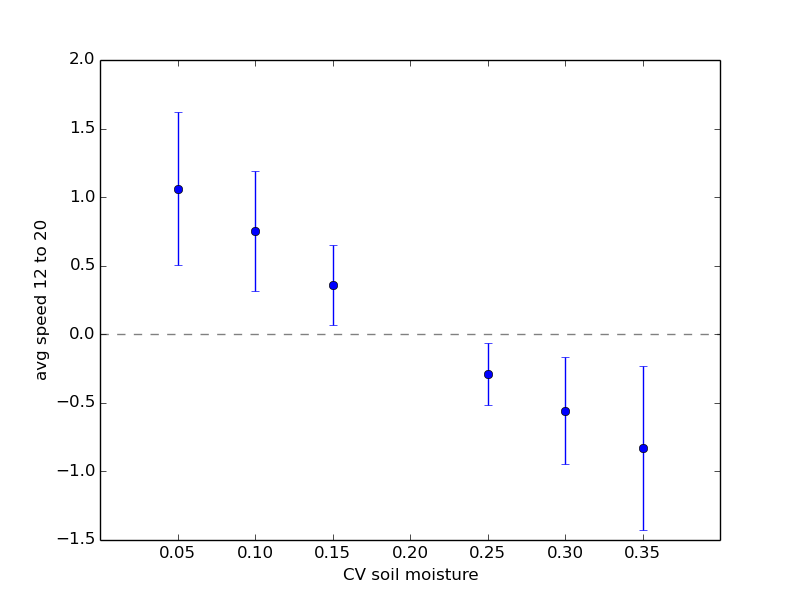
\includegraphics[width=1\textwidth]{ch3-wind/img/shifts_CVsmois_12-20_d02.png}
\caption{Average changes in wind speed between hours 12:00 and 20:00, for different values of CV soil moisture with CR and SN soil moisture set to 0.2 m$^3$/m$^3$.  Changes are relative to the CA-0.2 control case.  Error bars represent one standard deviation.}
\label{fig:windSol_ShiftsMaxCV}
\end{figure}

Drier Central Valley soils increase Solano winds, while wetter Central Valley soils decrease Solano winds, relative to the moderately wet control of soil moisture = 0.2 (Figure \ref{fig:windSol_TseriesWindCV}.)  These changes can be up to 3 m/s, and they occur most consistently in the hours of 12:00 to 22:00 (Figure \ref{fig:windSol_DiffDiurnalCV0pt2}(b)), when they are 0.8-1.7 m/s on average in the driest Central Valley case (CV0.05).  The average changes during hours 12:00 to 22:00 scale slightly nonlinearly with CV soil moisture (Figure \ref{fig:windSol_ShiftsMaxCV}), with larger increases in wind per unit soil moisture decrease when the Central Valley soil is drier than 0.2 m$^3$/m$^3$.  The greater sensitivity of wind to soil moisture when soils are drier may be due to a greater sensitivity of surface heating to soil moisture when soils are drier, because of rapid declines in soil hydraulic conductivity and plant stomatal conductance in the moderate-to-dry soil moisture range (\textbf{cite something � Bonan? Sap flow paper? Transitional soil moisture regime paper of some kind?}).

\clearpage

\subsection{Physical mechanism}
\label{subsec:PhysMech}

Next we investigate the physical mechanism by which changes in soil moisture, especially in the Central Valley, influence near-surface winds at Solano.  

The strong diurnal component of the Solano wind (Figures \ref{fig:windSol_TseriesDryRg} and \ref{fig:windSol_TseriesWetRg}) and the wind speed peak at low levels (Figure \ref{fig:windSol_VertProfileDryRg}) suggest significant forcing by land surface heating (consistent with Zhong \textit{et al.} [2004] and Mansbach [2010]).  In order to explore the influence of land surface forcing on terms in the momentum budget, we model the topographically channeled wind at Solano as simple one-dimensional flow through the pass governed by a one-dimensional momentum equation,

\begin{equation}
\frac{\partial u}{\partial t} = -u\frac{\partial u}{\partial x} -\frac{1}{\rho} \frac{\partial p}{\partial x} - F\left(\frac{\partial u}{\partial z}, N\right),
\label{eqn:windSol_momentum}
\end{equation}
neglecting the Coriolis term because of the topographic constraint on wind direction.  The first term on the right hand side is the advection of momentum, the second term is the pressure gradient force, and the third term is frictional dissipation as an unspecified function of vertical wind shear and stability (quantified by $N$, the Brunt-V\"ais\"al\"a frequency).  We are interested in the importance of each of these terms through the diurnal cycle and in the influence of soil moisture changes on each of these terms.

\subsubsection{Driving pressure gradient}

\begin{figure}[here]
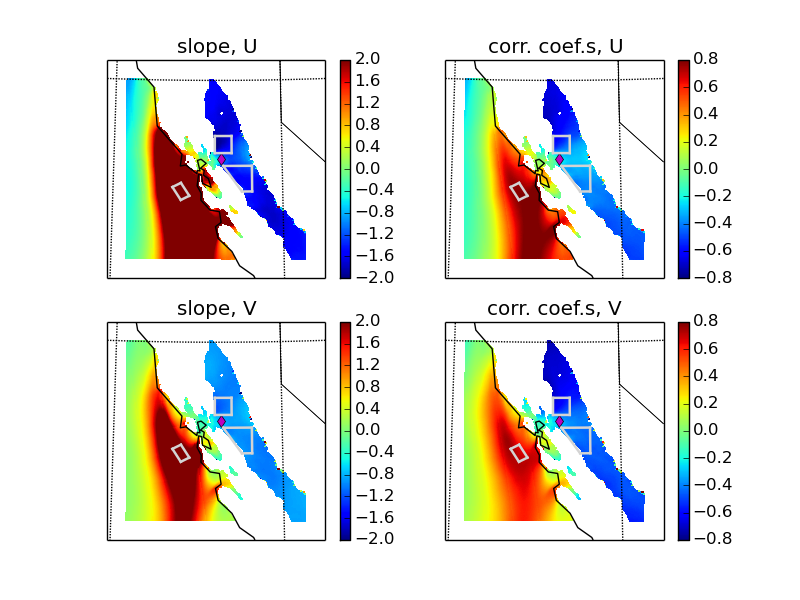
\includegraphics[width=1\textwidth]{ch3-wind/img/corr_wind_panom_lev110_lag12_CA0pt25.png}
\caption{CA-0.25 case: Solano 60 m AGL (110 m ASL) wind linearly regressed against horizontal pressure anomaly at 110 m ASL, with wind lagging pressure by 6 hours.  Top row: $u$-component of wind; bottom row: $v$-component of wind.  Left column: linear regression slope; right column: correlation coefficient.  Gray boxes outline areas used to calculate pressure gradients; ocean box is ``OCN", northern box in the Central valley is ``NCV", and southern box in Central Valley is ``SCV".}
\label{fig:windSol_CorrMap0pt25}
\end{figure}

\begin{figure}[here]
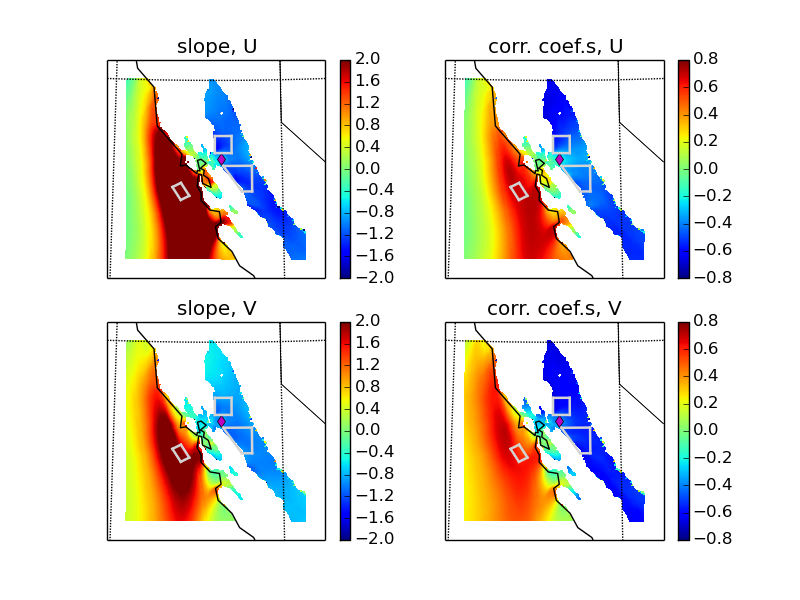
\includegraphics[width=1\textwidth]{ch3-wind/img/corr_wind_panom_lev110_lag12_CA0pt1.png}
\caption{CA-0.1 case: Solano 60 m AGL (110 m ASL) wind linearly regressed against horizontal pressure anomaly at 110 m ASL, with wind lagging pressure by 6 hours.  Top row: $u$-component of wind; bottom row: $v$-component of wind.  Left column: linear regression slope; right column: correlation coefficient.}
\label{fig:windSol_CorrMap0pt1}
\end{figure}

In order to identify the pressure gradient most relevant to Solano winds, we linearly regress the horizontal pressure anomaly, calculated at each output time step, against Solano turbine-level wind.  The regression is repeated for pressure at a range of heights and for a range of lag times, with wind lagging pressure.  The regression slopes and correlation coefficients for the control cases (CA-0.25, Figure \ref{fig:windSol_CorrMap0pt25}, and CA-0.1, Figure \ref{fig:windSol_CorrMap0pt1}) show a consistent pattern of positive slopes and correlation coefficients over the ocean near the central coast (meaning higher pressure in those regions corresponds to faster wind), and negative slopes and correlation coefficients throughout the Central Valley, especially just north and south of the Solano pass (meaning lower pressure in those regions corresponds to faster wind).

\begin{figure}[here]
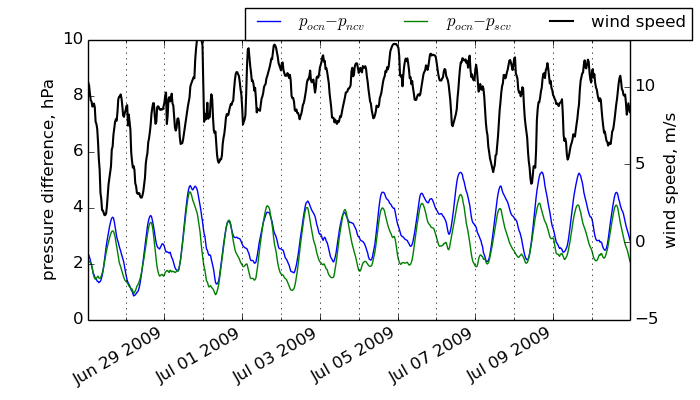
\includegraphics[width=1\textwidth]{ch3-wind/img/pgrad_wind_CA0pt1_level110.png}
\caption{CA-0.1 control case: Solano 60 m AGL (110 m ASL) wind (black) and average pressure difference OCN box minus NCV box (blue) and OCN box minus SCV box (green) at 110 m ASL.  The sign of the pressure difference is chosen to correspond with the $\frac{-1}{\rho} \frac{\partial p}{\partial x}$ term in the momentum budget.}
\label{fig:windSol_PgradWind}
\end{figure}

\begin{figure}[here]
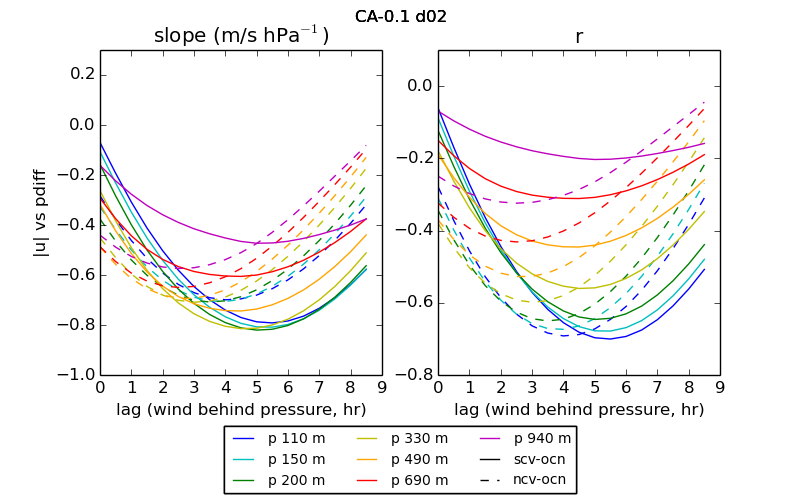
\includegraphics[width=1\textwidth]{ch3-wind/img/lag_corr_pdiff_combo_ncv_scv_d02_CA0pt1.png}
\caption{CA-0.1 control case: lagged linear regression of Solano 60 m AGL (110 m ASL) wind against average pressure difference NCV box minus OCN box (dashed) and SCV box minus OCN box (solid).  Correlations are only shown for speed, because u and v velocity component results are very similar.}
\label{fig:windSol_LagCorrCtrl}
\end{figure}

Based on this finding, we choose three boxes, shown in gray in Figures \ref{fig:windSol_CorrMap0pt25} to \ref{fig:windSol_CorrMap0pt1}, to represent the pressure gradient driving Solano winds.  The lag of wind speed behind pressure gradient is evident in the time series of Solano wind and pressure difference between the boxes (Figure \ref{fig:windSol_PgradWind}).  Not only does the pressure difference peak 5-6 hours before the Solano wind speed, but the peak pressure difference rapidly dissipates (beginning to decline after 1-2 hours), while the peak wind speed persists for 6-8 hours.  Using the pressure difference between the three boxes, we confirm that the peak sensitivity (as measured by the regression slope) and correlation occur with pressure at 110 m ASL (although the metrics are high at all levels below $\sim$300 m) with a lag of $\sim$4-5 hr for NCV-OCN pressure and $\sim$5-6.5 hr for SCV-OCN pressure (Figure \ref{fig:windSol_LagCorrCtrl}).

\begin{figure}[here]
\begin{subfigure}{0.6\textwidth}
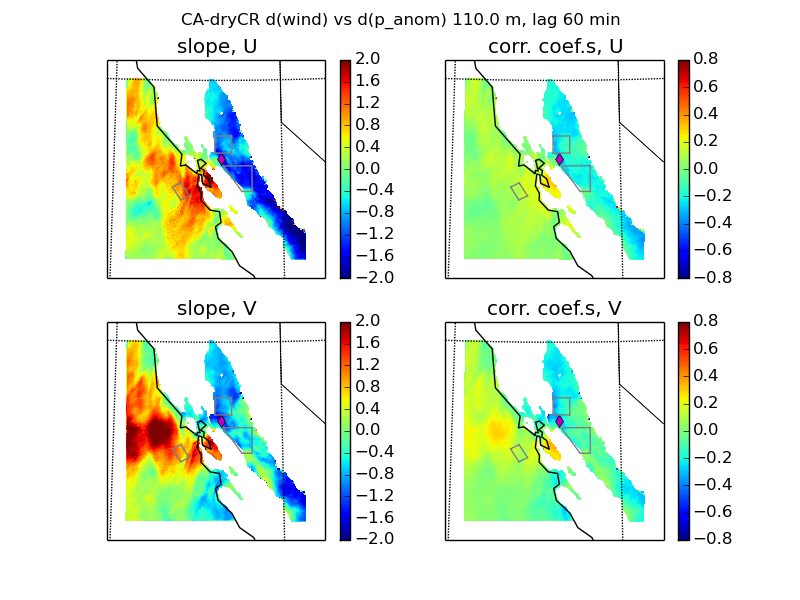
\includegraphics[width=\textwidth]{ch3-wind/img/corr_dwind_dpanom_lev110_lag2_dryCR.png}
\caption{}
\end{subfigure}
\begin{subfigure}{0.6\textwidth}
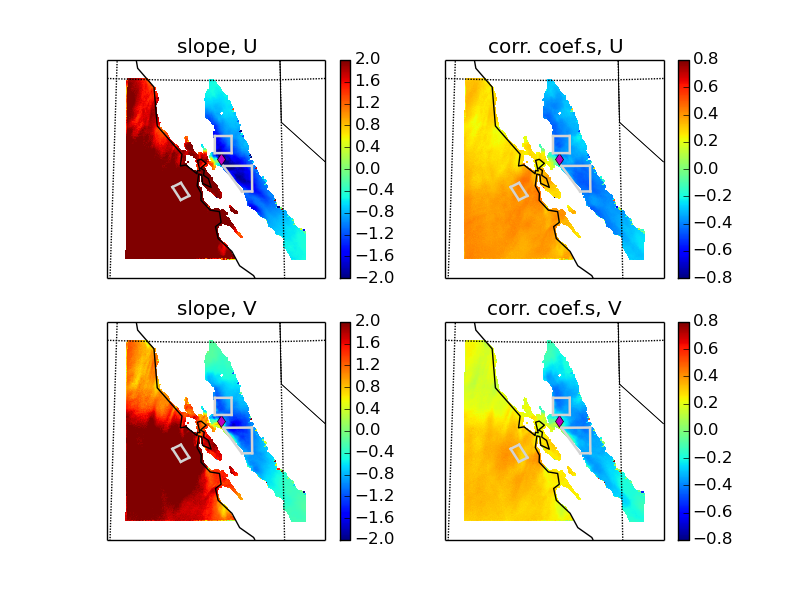
\includegraphics[width=\textwidth]{ch3-wind/img/corr_dwind_dpanom_lev110_lag2_dryCV.png}
\caption{}
\end{subfigure}
\begin{subfigure}{0.6\textwidth}
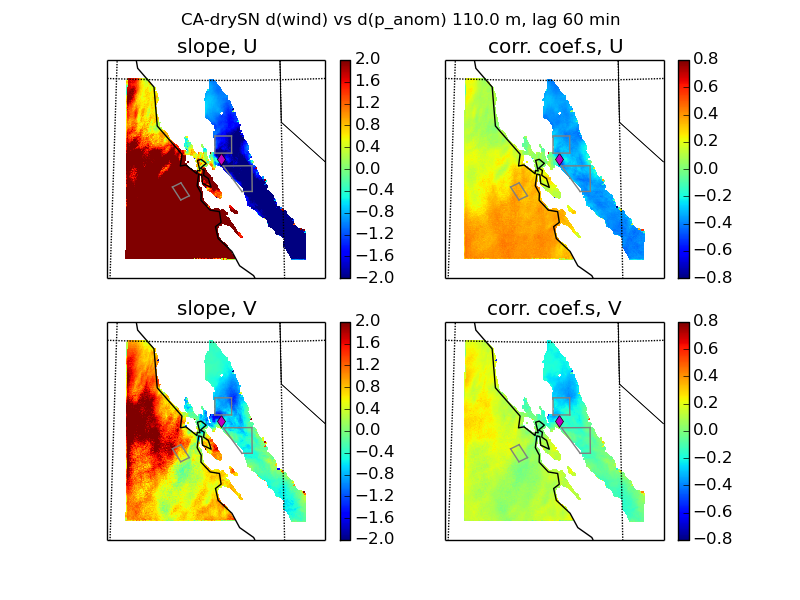
\includegraphics[width=\textwidth]{ch3-wind/img/corr_dwind_dpanom_lev110_lag2_drySN.png}
\caption{}
\end{subfigure}
\caption{Correlation between Solano wind changes at 60 m AGL and horizontal pressure anomaly of change in 110 m ASL pressure, with a lag of 60 min, for the dry regional test cases minus control: (a) dryCR, (b) dryCV, (c) drySN.  The order of panels is as in Figure \ref{fig:windSol_CorrMap0pt25}.}
\label{fig:windSol_CorrMapDryRg}
\end{figure}

\begin{figure}[here]
\begin{subfigure}{0.6\textwidth}
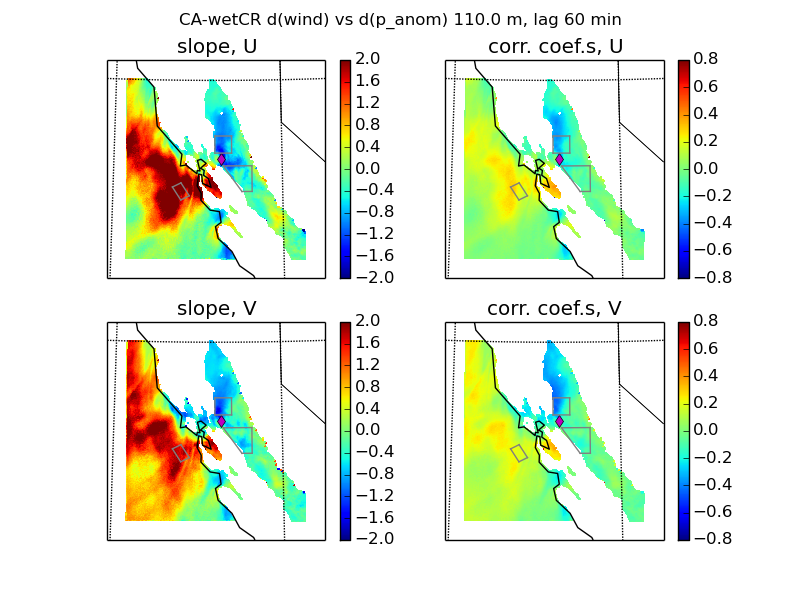
\includegraphics[width=\textwidth]{ch3-wind/img/corr_dwind_dpanom_lev110_lag2_wetCR.png}
\caption{}
\end{subfigure}
\begin{subfigure}{0.6\textwidth}
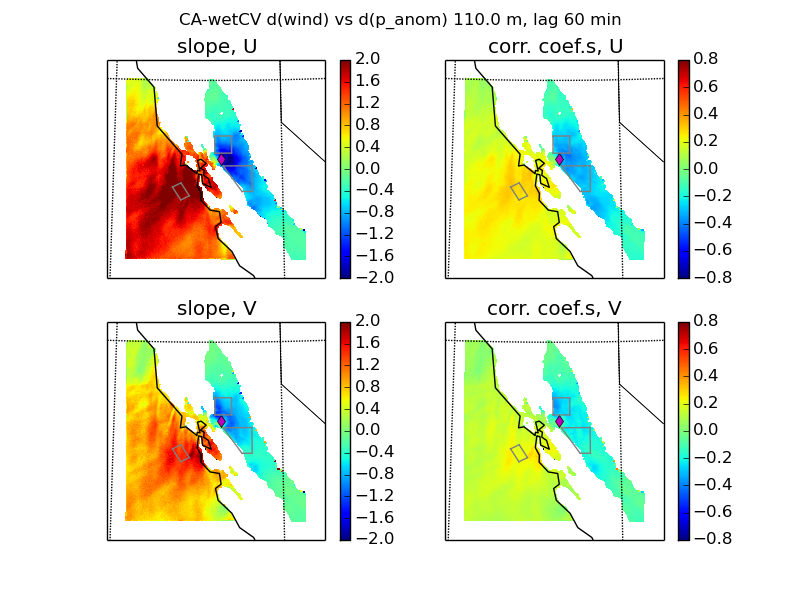
\includegraphics[width=\textwidth]{ch3-wind/img/corr_dwind_dpanom_lev110_lag2_wetCV.png}
\caption{}
\end{subfigure}
\begin{subfigure}{0.6\textwidth}
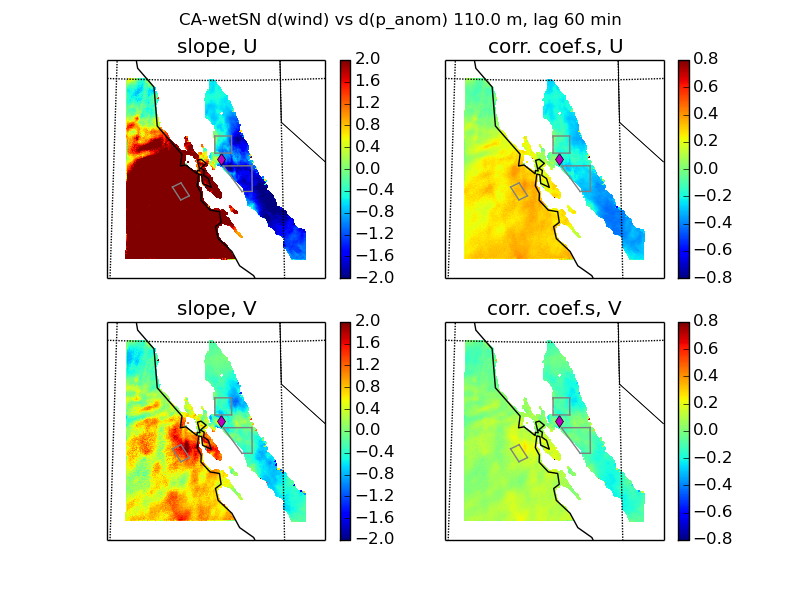
\includegraphics[width=\textwidth]{ch3-wind/img/corr_dwind_dpanom_lev110_lag2_wetSN.png}
\caption{}
\end{subfigure}
\caption{Correlation between Solano wind changes at 60 m AGL and horizontal pressure anomaly of change in 110 m ASL pressure, with a lag of 60 min, for the wet regional test cases minus control: (a) wetCR, (b) wetCV, (c) wetSN.  The order of panels is as in Figure \ref{fig:windSol_CorrMap0pt25}.}
\label{fig:windSol_CorrMapWetRg}
\end{figure}

\begin{figure}[here]
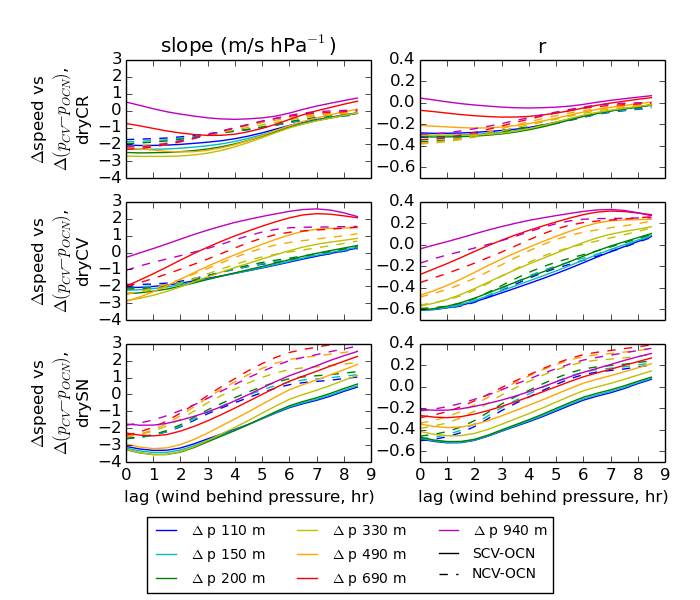
\includegraphics[width=1\textwidth]{ch3-wind/img/lag_corr_dpdiff_combo_ncv_scv_d02_testminusctrl.png}
\caption{Dry regional perturbation cases: lagged linear regression of test-minus-control Solano 60 m AGL (110 m ASL) wind against test-minus-control average pressure difference NCV box minus OCN box (dashed) and SCV box minus OCN box (solid).  Top row: dryCR; middle row: dryCV; bottom row: drySN.}
\label{fig:windSol_LagCorrTest}
\end{figure}

Repeating the regression analysis using test-minus-control changes in pressure and Solano wind, a similar spatial pattern of sensitivity emerges (positive correlation between Solano wind changes and pressure changes in the central coastal ocean, and negative correlation between Solano wind changes and pressure changes in the Central Valley), albeit with weaker correlation (Figures \ref{fig:windSol_CorrMapDryRg} and \ref{fig:windSol_CorrMapWetRg}).  Again, the changes in wind speed correlate maximally with the changes in pressure at the lowest altitudes ($\le$ 200 m, Figure \ref{fig:windSol_LagCorrTest}).  In contrast to the control cases which have a 5-6 hour lag, the test-minus-control changes correlate maximally at a lag of $\le$ 1 hour (Figure \ref{fig:windSol_LagCorrTest}).

\subsubsection{Temperature controls on pressure}

\begin{figure}[here]
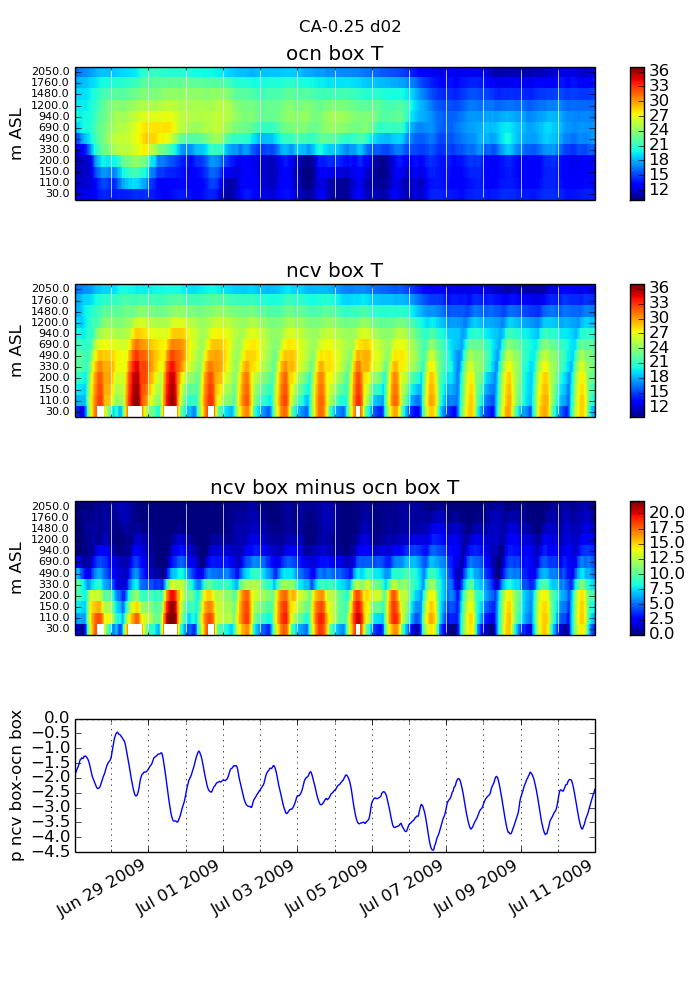
\includegraphics[width=0.9\textwidth]{ch3-wind/img/timeheight_T_pdiff_ocnbox_ncvbox_0pt25.png}
\caption{CA-0.25 control case: Temporal evolution of the vertical profile of temperature for the OCN box (top panel), the NCV box (second panel), NCV minus OCN (third panel); and time series of the NCV minus OCN pressure at 110 m ASL (bottom panel).  White areas indicate times when the lowest $\sigma$ model level was higher than 30 m ASL for the NCV box.}
\label{fig:windSol_TimeHeightCtrl}
\end{figure}

The diurnal variations in low-level pressure correspond to diurnal variations in boundary layer temperature, because pressure is the vertical integral of the weight of the air column above a point, and changes in temperature change the density and thus the weight of the air column.  Diurnal temperature variations are larger in the Central Valley than over the ocean (Figure \ref{fig:windSol_TimeHeightCtrl}).  In the NCV box, the temperature near the surface (\textless 100 m ASL) declines quickly after sunset, but the temperature aloft in the boundary layer (particularly 300-700 m) remains elevated until at least midnight (Figure \ref{fig:windSol_TimeHeightCtrl}, panel 2).  Both the NCV temperature and the NCV-OCN temperature difference peak around 17:00.  The temperature difference at low levels (\textless 110 m) drops after sunset and approaches zero in the early morning some days, but the temperature difference remains positive at 110-490 m on most days, with NCV warmer than OCN by up to 12 deg C even in the early morning.  The near-surface cooling in the Central Valley is due to a combination of radiative cooling of the land surface and advection of cooler marine air by the low-level wind maximum.  The pressure difference is most negative (strongest gradient) at the same time as the maximum temperature difference, around 17:00, and is smallest in magnitude (weakest gradient) just before sunrise, around 06:00, when the NCV boundary layer is coolest.  

\begin{figure}[here]
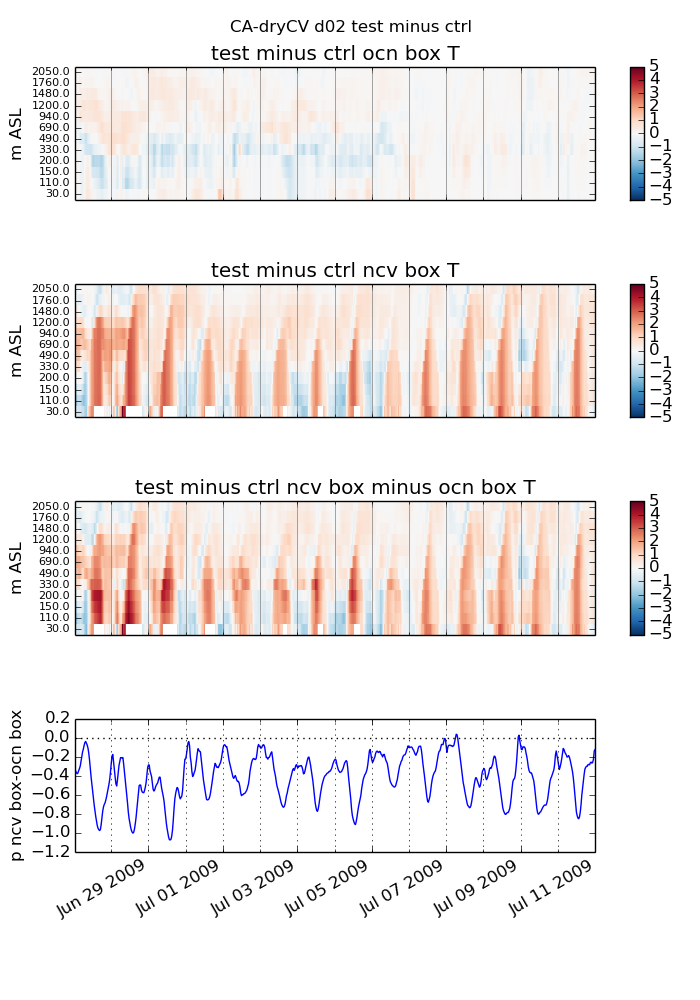
\includegraphics[width=0.9\textwidth]{ch3-wind/img/timeheight_T_pdiff_ocnbox_ncvbox_diff_dryCV.png}
\caption{dryCV case: Temporal evolution of the vertical profile of test-minus-control temperature changes for the OCN box (top panel), the NCV box (second panel), NCV minus OCN (third panel); and time series of test-minus-control changes in the NCV minus OCN pressure at 110 m ASL (bottom panel).  White areas indicate times when the lowest $\sigma$ model level was higher than 30 m ASL for the NCV box.}
\label{fig:windSol_TimeHeightDryCV}
\end{figure}

Changes in soil moisture affect the pressure gradient by changing surface heat fluxes and thus air temperature.  Temperature changes in the lower 1000 m of the NCV box are much larger in the dryCV case than in the dryCR or drySN cases; as such, only the dryCV case is shown (Figure \ref{fig:windSol_TimeHeightDryCV}).  We note that in the dryCR and drySN cases, temperature and pressure changes are much smaller (+/- 1 degree C and -0.4 hPa), and the pressure gradient strengthens in the late afternoon, largely corresponding to warming at boundary layer levels above the surface (150 m to 1200 m).

In the dryCV case, the NCV experiences strong low-level heating beginning in the morning, increasing in altitude as the boundary layer grows; temperature increases during day are well-mixed in the boundary layer.  There is mild cooling over the OCN box at 200-330 m in the first week of the simulation.  The strongest increase in temperature difference (warming of NCV relative to OCN) occurs late morning to late afternoon, at all levels below 690 m.  At night, there is a small decrease in the low-level (\textless 330 m) temperature difference.  The corresponding strengthening of the pressure difference is also greatest from late morning to late afternoon.  The mild strengthening of the pressure gradient on some nights (e.g. early morning of June 28, June 29, July 3, July 8) appears related to longer nocturnal persistence of warming at NCV relative to OCN in the residual boundary layer (150 m - 690 m, although the elevation of warming differs among individual days).

\subsubsection{Momentum budget timing and changes}

\begin{figure}[here]
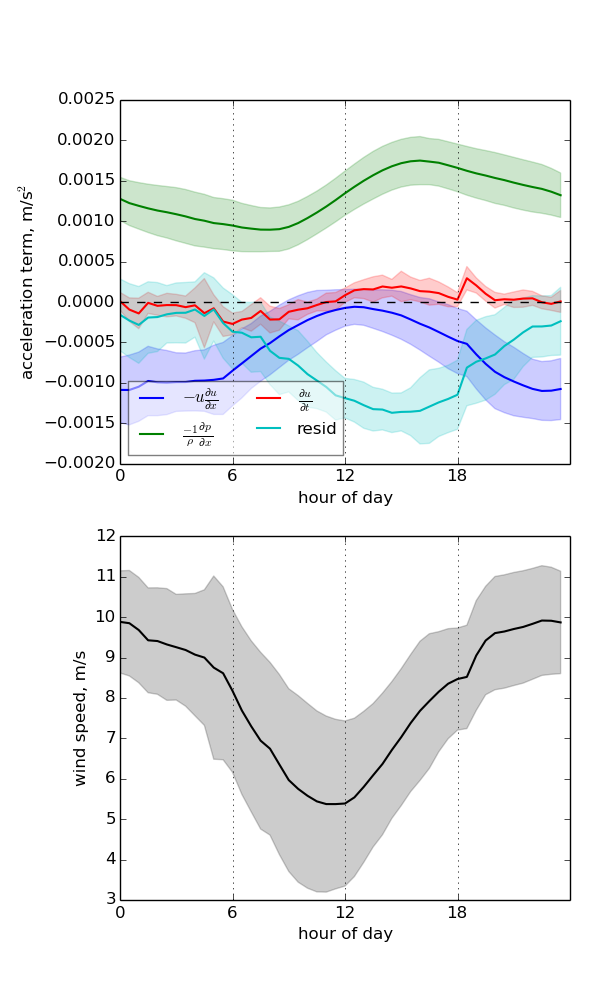
\includegraphics[width=0.9\textwidth]{ch3-wind/img/momentum_terms_diurnal_0pt25.png}
\caption{CA-0.25 control case: Diurnal average of terms of the momentum balance.  Pressure gradient is calculated between the NCV and OCN boxes, and using density calculated at Solano 60 m AGL.  Advection is calculated as $u_{solano}\frac{\partial u}{\partial x}$ with $\frac{\partial u}{\partial x}$ estimated with the gradient in wind between Solano and San Pablo Bay (the northern part of the San Francisco Bay).  $\frac{\partial u}{\partial t}$ is calculated using Solano 60 m AGL wind speed.  Friction (cyan) is calculated as the residual of the other three terms, following Equation \ref{eqn:windSol_momentum}.  Shading represents one standard deviation.}
\label{fig:windSol_MomTermsDiurn}
\end{figure}

The momentum advection, pressure gradient, and $u$ time tendency terms in Equation \ref{eqn:windSol_momentum} are estimated from model output for the CA-0.25 control (Figure \ref{fig:windSol_MomTermsDiurn}).  Using these three model-derived terms, we calculate the friction term as the residual (Figure \ref{fig:windSol_MomTermsDiurn}, cyan line).  The friction term has to vary diurnally in order to reproduce the observed wind diurnal cycle.  The time tendency ($\frac{\partial u}{\partial t}$) term is much smaller than pressure gradient term, even in afternoon when the pressure gradient is largest and advection is small.  If friction were not also large at this time, the wind would accelerate much faster.  Conversely, high wind speeds persist even after the pressure gradient declines between 22:00 and 04:00 and despite the strong advection of lower momentum air.  If friction during the night remained at its high afternoon values, the winds would decelerate at night.  The decline in the friction term at night is necessary in order to explain the observed high winds at night.  [\textbf{cite LLJ paper of some sort - not the first time this is being said.}]  Moreover, this residual has the expected diurnal shape of friction, with high values in the daytime when convective turbulence creates a uniform boundary layer and high momentum flux to the ground, and low values at night when the residual upper boundary layer decouples from the shallow stable nocturnal boundary layer and is buffered from friction with the surface.
% Indeed, the diurnal course of modeled $u*$ at Solano has the same timing as the $F(\frac{\partial u}{\partial z}, N)$ term calculated from the residual (ustar figure).

\begin{figure}[here]
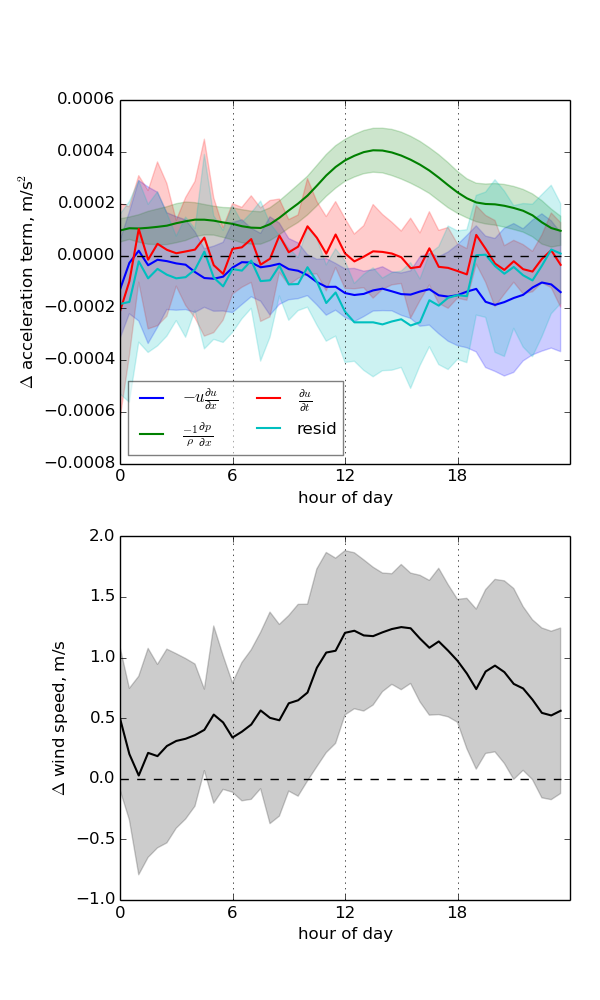
\includegraphics[width=0.9\textwidth]{ch3-wind/img/momentum_terms_diurnal_diff_dryCV.png}
\caption{dryCV case: Diurnal average of test-minus-control change in terms of the momentum balance, calculated as in Figure \ref{fig:windSol_MomTermsDiurn}.  Shading represents one standard deviation.}
\label{fig:windSol_MomTermsDiurnDiff}
\end{figure}

In the dryCV case, the pressure gradient term increases at all hours but especially between 10:00 and 18:00 (Figure \ref{fig:windSol_MomTermsDiurnDiff}), when it increases by 20\% to 30\% (cf. Figure \ref{fig:windSol_MomTermsDiurn}).  The advection term becomes more negative at those same hours, as faster Solano wind transports lower momentum air more effectively.  The friction term also becomes more negative in the daytime, probably due to greater instability and convection from the hotter Central Valley land surface.  The changes in the dryCR and drySN cases were much smaller, with the pressure gradient term increasing by a maximum of 0.0001 to 0.0002 m/s$^2$ in the late afternoon.

\subsubsection{Summary of mechanism}
Solano wind responds to the near-surface pressure gradient between the Central Valley near the Solano pass and the central coast ocean.  Changes in boundary layer temperature at either of these locations influences this driving pressure gradient.  Soil moisture strongly influences land surface heating, and changes to soil moisture in the Central Valley strongly affect boundary layer temperature and thus near-surface pressure in the regions relevant to the Solano wind.  When Central Valley soils are dry, the atmospheric boundary layer warms from late morning to late afternoon, strengthening the pressure gradient at those hours.  At the same time, friction and advection of lower momentum air increase, due respectively to increased convection and faster lateral transport.  These negative terms limit the increase of Solano winds to $\sim$1.5 m/s on average in the late afternoon.

%\end{document}